\documentclass[18pt]{beamer}
\usepackage[utf8]{inputenc} % for the umlauts
\usepackage{subfigure}

\beamertemplatenavigationsymbolsempty
%% SLIDE FORMAT

% use 'beamerthemekit' for standard 4:3 ratio
% for widescreen slides (16:9), use 'beamerthemekitwide'

\usepackage{templates/beamerthemekit}
\usepackage{stackengine}
\usepackage{graphicx}
% \usepackage{templates/beamerthemekitwide}

\setcounter{tocdepth}{1}

%% TITLE PICTURE

% if a custom picture is to be used on the title page, copy it into the 'logos'
% directory, in the line below, replace 'mypicture' with the 
% filename (without extension) and uncomment the following line
% (picture proportions: 63 : 20 for standard, 169 : 40 for wide
% *.eps format if you use latex+dvips+ps2pdf, 
% *.jpg/*.png/*.pdf if you use pdflatex)

%\titleimage{mypicture}

%% TikZ INTEGRATION

% use these packages for PCM symbols and UML classes
% \usepackage{templates/tikzkit}
% \usepackage{templates/tikzuml}

% the presentation starts here

\usepackage[absolute,overlay]{textpos}
%\usepackage[texcoord,grid,gridunit=mm,gridcolor=red, subgridcolor=green]{eso-pic}
\setbeamercovered{invisible}

\title[SWT1]{Softwaretechnik 1 - 1. Tutorium}
\subtitle{Tutorium 18}
\author{Felix Bachmann}
\date{08.05.2018}

\institute{KIT - Institut für Programmstrukturen und Datenorganisation (IPD)}

% Bibliography

\usepackage[citestyle=authoryear,bibstyle=numeric,hyperref,backend=biber]{biblatex}
\addbibresource{templates/example.bib}
\bibhang1em

\begin{document}

% change the following line to "ngerman" for German style date and logos
\selectlanguage{ngerman}

%title page
\begin{frame}
\titlepage
\end{frame}

%table of contents
\begin{frame}{Themenübersicht}
\tableofcontents
\end{frame}

\section{Orga}
	\subsection{Feedback 1. Übungsblatt}
	\begin{frame}
		\frametitle{1. Übungsblatt Statistik}
		%TODO
		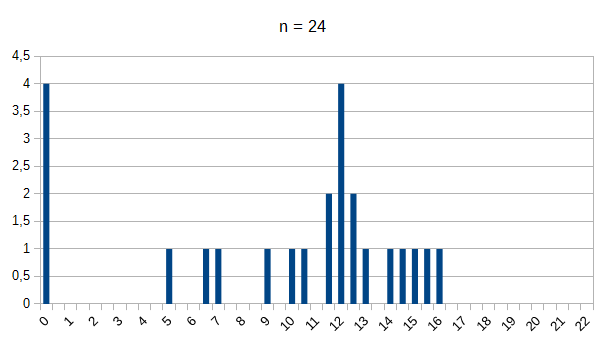
\includegraphics[scale=0.7]{./pics/tut1/statistics_ub1.png}
	\end{frame}
	
	\subsection{1. Übungsblatt - Fehler (Allgemein)}
	\begin{frame}
		\frametitle{Häufige Fehler}
		%TODO
		\begin{block}{Allgemein}
			generell ohne Abzug:
			\begin{itemize}
				\item gleiche Abgabe bei allen Aufgaben
			\end{itemize}
			generell mit Abzug: (bis zu -2P)
			\begin{itemize}
				\item  CheckStyle nicht beachtet
				\item JavaDoc nicht vollständig / nicht aussagekräftig
				\item zu wenige commits / nicht aussagekräftige commit-messages
			\end{itemize}
		\end{block}
	\end{frame}
	
	\subsection{1. Übungsblatt - Fehler (Aufgabe 1)}
	\begin{frame}
		\frametitle{Häufige Fehler}
		%TODO
		\begin{block}{Aufgabe 1 (Altsoftware vorbereiten)}
		\begin{itemize}
			\item *.properties falsch / nicht verschoben (ist Ressource!)
			\item in src.xml wurden *.launch-Dateien nicht hinzugefügt
		\end{itemize}
		\end{block}
	\end{frame}
	
	\subsection{1. Übungsblatt - Fehler (Aufgabe 2)}
	\begin{frame}
		\frametitle{Häufige Fehler}
		%TODO
		\begin{block}{Aufgabe 2 + 3 (Modultests + Testüberdeckung)}
			\begin{itemize}
				\item auch bei Drehung um 0$^{\circ}$  ist Überprüfung des Bildes nötig (Dimensionen + Pixel) \pause
				\item equals() reicht nicht aus, um Gleichheit der Bilder zu prüfen \pause 
				\item new File() erstellt kein File, sondern nur einen "'pointer"' auf einen Pfad (siehe File.createNewFile() oder File.mkdir()) \pause
				\item benutzt relative Pfade (beginnen im jmjrst.main-Ordner) \pause 
				\item Testklasse in gleiches Paket wie zu testenden Klasse \pause 
				\item fügt Abhängigkeiten in die jmjrst.main-pom.xml ein, \textbf{nicht} in die von iMage 
			\end{itemize}
		\end{block}
	\end{frame}

\section{Wasserfallmodell}
	\subsection{Wasserfallmodell, ohne Grafik}
	\begin{frame}
		\frametitle{Wasserfallmodell}
		\begin{itemize}
			\item Was ist das? 
		\end{itemize}
	\end{frame}
	
	\subsection{Wasserfallmodell, mit Grafik}
	\begin{frame}
		\frametitle{Wasserfallmodell}
		\begin{itemize}
			\item \textcolor{red}{dokumentengetriebenes Prozessmodell} \pause
			\item mögliche Phasen der Softwareentwicklung \pause
		\end{itemize}
		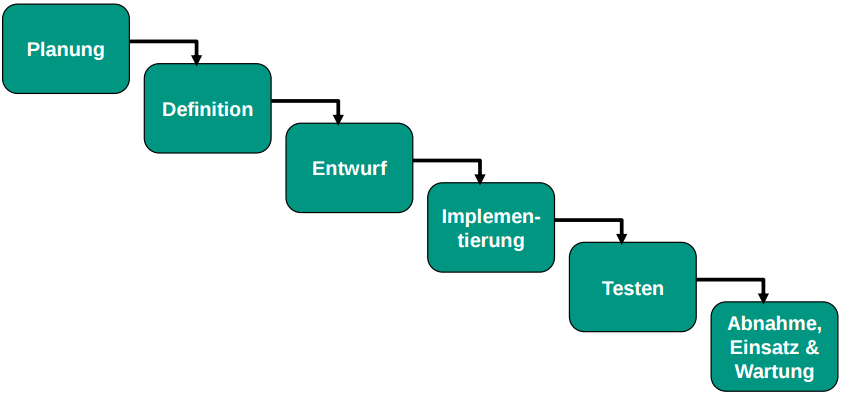
\includegraphics[scale=0.4]{./pics/tut1/waterfall_without-docs.png}
	\end{frame}
	
	\subsection{Wasserfallmodell, mit Grafik und Dokumenten}
	\begin{frame}
		\frametitle{Wasserfallmodell}
		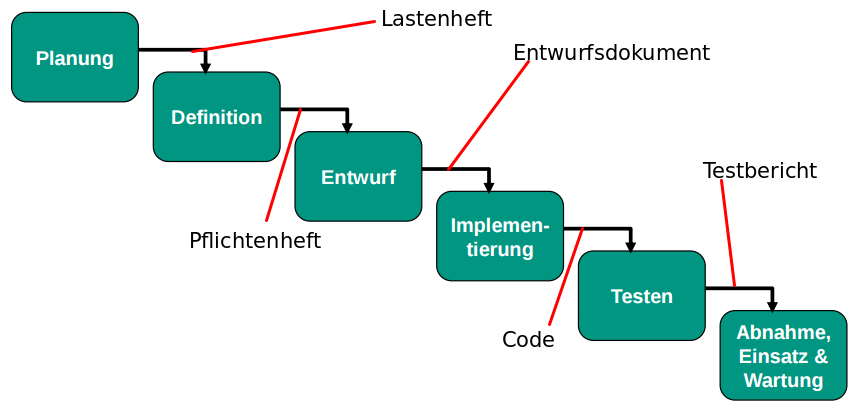
\includegraphics[scale=0.4]{./pics/tut1/waterfall_with-docs.png}
		\pause
		Dokumente für das 2. ÜB: 
		\begin{itemize}
			\item Lastenheft
			\item Durchführbarkeitsuntersuchung (weiteres Artefakt der Planung)
		\end{itemize}
	\end{frame}

\section{Durchführbarkeitsuntersuchung}
	\subsection{Welche Aspekte?}
	\begin{frame}
		\frametitle{Durchführbarkeitsuntersuchung - Gliederung}
		\begin{block}{Grundlegende Frage}
			Ist das Projekt in dem jeweiligen Szenario überhaupt durchführbar?
		\end{block}
		\begin{enumerate}
			\item \pause Fachlich \pause (softwaretechnisch leicht realisierbar?) \pause
			\item Alternativen \pause (lieber altes Projekt anpassen oder komplett neu entwickeln?) \pause
			\item Personell \pause (genug qualifizertes Personal?) \pause
			\item Risiken \pause (Gibt es Risiken? :D) \pause
			\item Ökonomisch \pause (wirtschaftlich? Termine?) \pause
			\item Rechtlich \pause (Datenschutz, Standards)
		\end{enumerate}
		\pause
		\begin{alertblock}{Fürs Übungsblatt}
			Denkt euch was (plausibles) aus!
		\end{alertblock}
	\end{frame}

\section{Lastenheft}
	\subsection{Lastenheft - Gliederung}
	\begin{frame}
		\frametitle{Lastenheft - Gliederung}
		\begin{block}{Grundlegende Aufgabe}
			Das Lastenheft sammelt die Anforderungen des Auftraggebers an den Auftragnehmer.
		\end{block}
		\begin{enumerate}
			\item \pause Zielbestimmung (grobe Beschreibung) \pause 
			\item Produkteinsatz (Für wen? Zielgruppe, Anwendungsbereich)\pause
			\item Funktionale Anforderungen (feingranular: Funktionen des Produkts)\pause 
			\item Produktdaten (Welche Daten speichern?)\pause
			\item Nichtfunktionale Anforderungen (Meta-Anforderungen: Zeit, Zuverlässigkeit)\pause 
			\item Systemmodelle
			\begin{itemize}
				\item Szenarien (spezielles Beispiel)
				\item Anwendungsfälle (allgemeiner Verwendungszweck)
			\end{itemize}
			\pause
			\item Glossar (technische Begriffe erklären)
		\end{enumerate}
	\end{frame}
	
	\subsection{Lastenheft - Unterschiede}
	\begin{frame}
		\frametitle{Begriffsklärung}
		\begin{block}{Zielbestimmung vs. Funktionale Anforderungen}
			\pause
			\begin{itemize}
				\item Zielbestimmung: allgemeine Beschreibung, was das Produkt können soll
				\item Funktionale Anforderungen: konkrete Auflistung von Funktionen
			\end{itemize}
		\end{block}
		\pause
		\begin{block}{Funktionale Anforderungen vs. Nichtfunktionale Anforderungen}
			\pause
			\begin{itemize}
				\item Funktionale Anforderungen: Funktionen des Produkts
				\item Nichtfunktionale Anforderungen: "'Meta"'-Eigenschaften des Produkts
			\end{itemize}
		\end{block}
		\pause
		\begin{block}{Zielbestimmung vs. Produkteinsatz}
			\pause
			\begin{itemize}
				\item Zielbestimmung: allgemeine Beschreibung, was das Produkt können soll
				\item Produkteinsatz: Rahmenbedingungen (Zielgruppe, Anwendungsbereiche)
			\end{itemize}
		\end{block}
	\end{frame}
	
\section{Pflichtenheft}
	\subsection{Pflichtenheft - Aufgabe}
	\begin{frame}
		\frametitle{Wozu ein Pflichtenheft?}
		\begin{block}{Grundlegende Aufgabe}
			Erweiterung des Lastenheftes, sodass exakt abgebildet ist \textbf{was} (noch nicht \textbf{wie}) zu implementieren ist.
		\end{block}
	\end{frame}
	
	\subsection{Pflichtenheft - Gliederung}
	\begin{frame}
		\frametitle{Pflichtenheft - Gliederung}
		\pause
		\begin{enumerate}
			\item Zielbestimmung  
			\item Produkteinsatz 
			\item \underline{\textbf{Produktumgebung}} (Hard-/Software in Einsatzumgebung)
			\item Funktionale Anforderungen 
			\item Produktdaten 
			\item Nichtfunktionale Anforderungen 
			\item \underline{\textbf{Globale Testfälle}} (\enquote{zu testende Abläufe})
			\item Systemmodelle
			\begin{itemize}
				\item Szenarien
				\item Anwendungsfälle
				\item \underline{\textbf{Objektmodelle}} $\implies$ UML-Klassendiagramme (heute)
				\item \underline{\textbf{Dynamische Modelle}} $\implies$ nächstes Mal
				\item \underline{\textbf{Benutzerschnittstelle}} $\implies$ Zeichnungen/Screenshots
			\end{itemize}
			\item Glossar 
		\end{enumerate}
	\end{frame}
	
	\subsection{Lastenheft - Unterschiede}
	\begin{frame}
		\frametitle{Begriffsklärung}
		\begin{block}{Produkteinsatz vs. Produktumgebung}
			\pause
			\begin{itemize}
				\item Produkteinsatz: Rahmenbedingungen (Zielgruppe, Anwendungsbereiche)
				\item Produktumgebung: Rahmenbedingungen bzgl. Software/Hardware
			\end{itemize}
		\end{block}
	\end{frame}
	
	\subsection{Quiz}
	\begin{frame}
		\frametitle{Quiz (Ankreuzaufgaben aus Klausuren)}
		Wahr oder falsch?
		\begin{itemize}
			\item Das Lastenheft ist eine Verfeinerung des Pflichtenheftes. \pause \colorbox{red}{falsch} \pause
			\item Das Lastenheft ist das Ergebnis der Planungsphase. \pause \colorbox{green}{wahr} \pause
			\item Nicht-funktionale Eigenschaften beschreiben, was das Produkt nicht tun sollte. \pause \colorbox{red}{falsch} \pause 
			\item Das Pflichtenheft beschreibt nur, was zu implementieren ist und nicht wie. \pause \colorbox{green}{wahr} \pause 
			\item Nicht-funktionale Anforderungen sind sowohl Teil des Pflichtenhefts als auch des Lastenhefts. \pause \colorbox{green}{wahr}
		\end{itemize}
		
	\end{frame}

\section{UML-Klassendiagramm}
	\subsection{UML? Kann man das essen?}
	\begin{frame}
		\frametitle{UML? Kann man das essen?}
		\begin{itemize}
			\item UML = \textbf{U}nified \textbf{M}odeling \textbf{L}anguage
			\item grafische Modellierungssprache, strenge Syntax
		\end{itemize}
		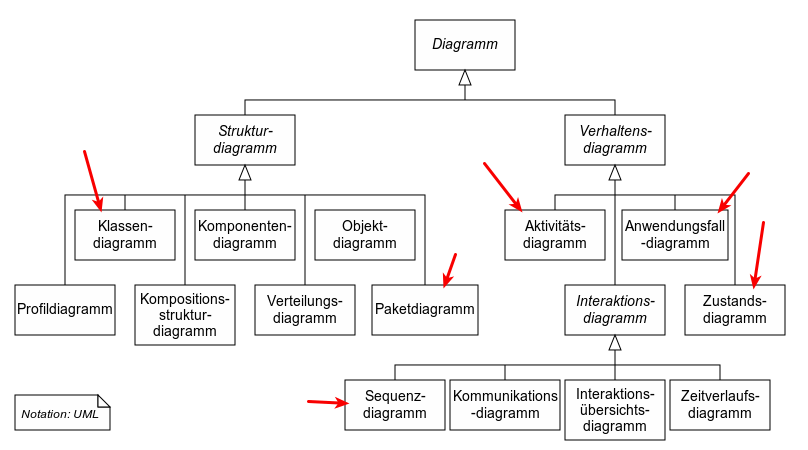
\includegraphics[scale=0.35]{./pics/tut1/uml_diagrams.png}
	\end{frame}	
	
	\subsection{UML-Klassendiagramm (1)}
	\begin{frame}
		\frametitle{UML-Klassendiagramm: Klassen + Vererbung}
		\centering
		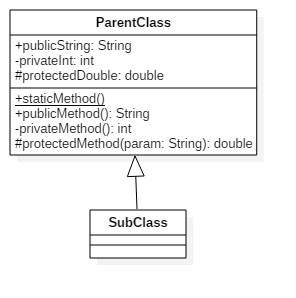
\includegraphics[scale=0.5]{./pics/tut1/inheritence.png}
		\pause
		\begin{small}
			\begin{itemize}
				\item - ist private: von Instanzen derselben Klasse sichtbar (\textcolor{red}{aber von allen!})
			\end{itemize}
		\end{small}
	\end{frame}
	
	\subsection{UML-Klassendiagramm (2)}
	\begin{frame}
		\frametitle{UML-Klassendiagramm: Interface}
		\centering
		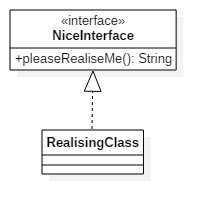
\includegraphics[scale=0.7]{./pics/tut1/interface.png}
	\end{frame}
	
	\subsection{UML-Klassendiagramm (3)}
	\begin{frame}
		\frametitle{UML-Klassendiagramm: Abstrakte Klassen}
		\begin{figure}
			\footnotesize
			\stackunder{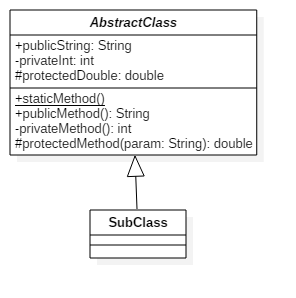
\includegraphics[scale=0.5]{./pics/tut1/abstract.png}}{UML-Notation} \pause
			\stackunder{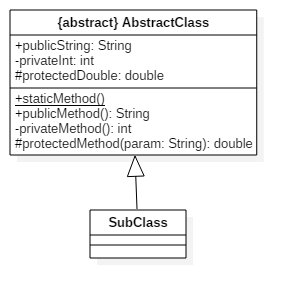
\includegraphics[scale=0.5]{./pics/tut1/abstractUb.png}}{Notation für Abgaben}
		\end{figure}
		\centering \textcolor{red}{Kursiv schriftlich nicht erkennbar!}
	\end{frame}
	
	\subsection{UML-Klassendiagramm (4)}
	\begin{frame}
		\frametitle{UML-Klassendiagramm: Assoziationen}
		\begin{figure}
			\footnotesize
			\stackunder{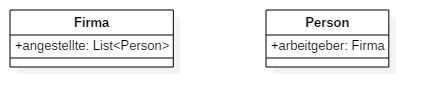
\includegraphics[scale=0.5]{./pics/tut1/wrong_assoc.png}}{so nicht,\dots} \pause
			\stackunder{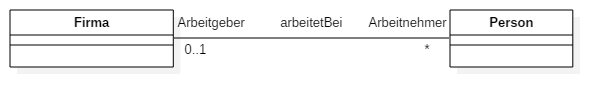
\includegraphics[scale=0.5]{./pics/tut1/correct_assoc.png}}{\dots, sondern so}
		\end{figure}
		\pause
		\begin{block}{UML}
			Beziehungen sollen direkt ersichtlich werden\linebreak
			$\implies$nur primitive Typen als Felder
		\end{block}
	\end{frame}
	
	\subsection{UML-Klassendiagramm (5)}
	\begin{frame}
		\frametitle{UML-Klassendiagramm: Aggregation + Komposition}
		\begin{figure}
			\footnotesize
			\stackunder{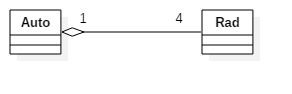
\includegraphics[scale=0.5]{./pics/tut1/aggregation.png}}{Aggregation} \pause
			\stackunder{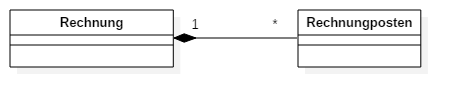
\includegraphics[scale=0.5]{./pics/tut1/composition.png}}{Komposition}
		\end{figure}
	\end{frame}
	
	\subsection{UML-Klassendiagramm(6)}
	\begin{frame}
		\frametitle{Aggregation vs Komposition}
		\begin{alertblock}{Unterschied}
			\begin{itemize}
				\item Aggregation: Teil-Ganzes-Beziehung
				\item Komposition: Aggregation, Teil kann ohne Ganzes nicht existieren
			\end{itemize}
		\end{alertblock}
	\end{frame}
	
	\subsection{UML-Klausuraufgabe(1)}
	\begin{frame}
		\frametitle{Klausuraufgabe SS09}
		\textit{Modellieren Sie das Szenario möglichst vollständig als UML-Klassendiagramm. Modellieren Sie keine Methoden. Geben Sie Attribute, Multiplizitäten, Restriktionen, Assoziationsnamen sowie Rollen an.} \linebreak
		Ein Fachwerkhaus besteht aus 5 bis 10 Holzstämmen, 200 bis 400 Lehmziegeln sowie 1.000 bis 2.000 Nägeln. Jedes Baumaterial, egal ob Holzstamm, Lehmziegel oder Nagel, ist Bestandteil in genau einem Fachwerkhaus. Jedes Fachwerkhaus hat eine bestimmte Anzahl an Zimmern und Stockwerken. Für den Bau eines Fachwerkhauses ist mindestens ein Zimmermann zuständig, welcher einen Namen sowie einen individuellen Stundenlohn besitzt. Zum Bau des Fachwerkhauses verwendet jeder Zimmermann sein eigenes Werkzeug, bestehend aus genau einem Hammer sowie genau einer Säge. Jeder Zimmermann kann an maximal einem Fachwerkhaus gleichzeitig bauen. 
	\end{frame}
	
	\subsection{UML-Klausuraufgabe(2)}
	\begin{frame}
		\frametitle{Musterlösung}
		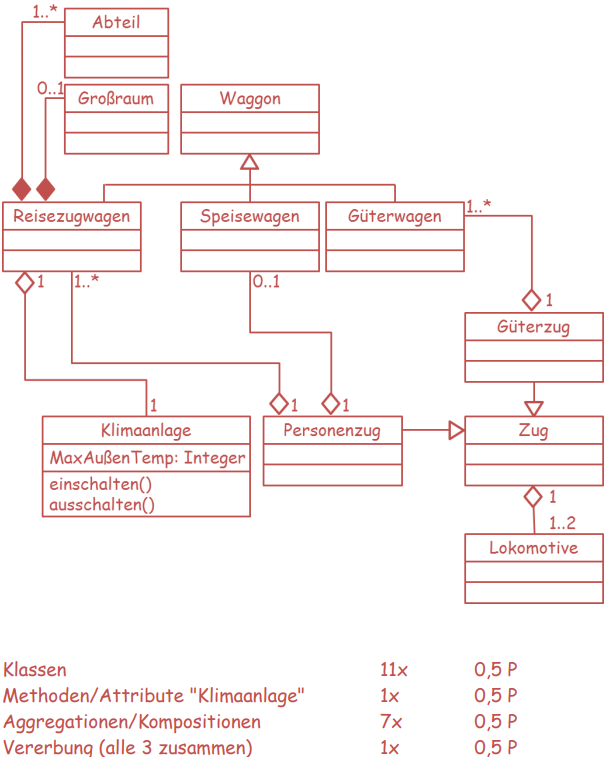
\includegraphics[scale=0.48]{./pics/tut1/solution.png}
	\end{frame}
		
		
\section{\LaTeX}
	\subsection{Basics}
	\begin{frame}
		\frametitle{\LaTeX - Basics}
		\begin{itemize}
			\item auf dem Blatt müsst ihr \LaTeX  ~ für die Dokumente benutzen
			\item nicht wie z.B. Word WYSIWYG, sondern WYSIWYAF / WYSIWYM
			\item wird euch an der Uni immer wieder begegnen, oft Pflicht
			\pause
			\item Vorteile:
			\begin{itemize}
				\item gut versionierbar
				\item leicht Formeln erstellbar
				\item nach Eingewöhnung recht intuitiv (vergleichbar mit HTML)
				\item multifunktional (Dokumente, Präsentationen, \dots)
			\end{itemize}
			\pause
			\item Nachteile:
			\begin{itemize}
				\item Einarbeitung notwendig :(
			\end{itemize}
		\end{itemize}
	\end{frame}
	
	\subsection{Installation}
	\begin{frame}
		\frametitle{\LaTeX - Installation}
		Installation einer Distribution notwendig, z.B.:
		\begin{itemize}
			\item  MiKTeX für Windows
			\item TeX Live für Linux, Mac, Windows
		\end{itemize}
		\pause
		Editoren machen das Schreiben von \LaTeX -Dokumenten angenehmer
		\begin{itemize}
			\item Texmaker
			\item TeXstudio (erweiterter Texmaker, mein Favorit)
			\item TeXclipse (Plugin für Eclipse)
			\item \dots
		\end{itemize}
	\end{frame}
	
	\subsection{Beispiel}
	\begin{frame}
		\frametitle{\LaTeX - Beispiel}
		\centering \huge Beispiel
	\end{frame}
		
\section{Tipps}
	\subsection{Tipps}
	\begin{frame}
		\frametitle{Tipps - 2. Übungsblatt}
		\begin{small}
			\begin{exampleblock}{Aufgabe 1 + 3: Lastenheft + Durchführbarkeitsuntersuchung}
				\begin{itemize}
					\item lasst euch was (sinnvolles) einfallen
					\item benutzt \LaTeX
				\end{itemize}
			\end{exampleblock}
			\pause
			\begin{exampleblock}{Aufgabe 2: Klassendiagramme}
				\begin{itemize}
					\item achtet auf Schlüsselwörter ("'ist ein"', "'enthält ein"', "'besteht aus"',\dots)
				\end{itemize}
			\end{exampleblock}
			\pause
			\begin{exampleblock}{Aufgabe 4 + 5: Geometrify + cmd-Programm}
				\begin{itemize}
					\item an einigen Stellen sind Aufgaben etwas vage
					\linebreak $\implies$ überlegt euch, was Sinn macht
				\end{itemize}
			\end{exampleblock}
		\end{small}
	\end{frame}
	
	\subsection{Abgabe}
	\begin{frame}
		\frametitle{Denkt dran!}
		%TODO
		\begin{alertblock}{Abgabe}
			\begin{itemize}
				\item Deadline am 24.5 um 12:00
				\item Dokumente ausdrucken
				\item Klassendiagramme handschriftlich
			\end{itemize}
		\end{alertblock}
	\end{frame}
		
	\begin{frame}
		\frametitle{Bis dann! (dann := 22.05.18)}
		\centering
		
\includegraphics[scale=0.86]{./comics/geek_and_poke_javadoc.jpg}
	\end{frame}

\end{document}
